\documentclass{article}

% Add search paths for input files
\makeatletter
\def\input@path{{../../../artisynth_core/doc/}{../../../artisynth_core/}{../../../artisynth_core/doc/texinputs/}}
\makeatother

\usepackage{amsmath}
\usepackage{framed}

%\usepackage{layout}
%\usepackage{showframe}
\input{artisynthDoc}
%\input{mathdefs}

\newcommand{\AS}{<ArtisynthRoot>}
\newcommand{\AM}{<ArtisynthModels>}
\newcommand{\BS}{<BatchsimRoot>}
\newcommand{\BM}{{\tt BatchManager}}
\newcommand{\BW}{{\tt BatchWorker}}
\newcommand{\BWs}{{\tt BatchWorkers}}

\begin{document}

\setcounter{tocdepth}{5}
\setcounter{secnumdepth}{3}

\title{The Batch Simulation Framework}
\author{Francois Roewer-Despres}
\setpubdate{Last update: Apr 26, 2018}

\iflatexml
\date{}
\fi

\maketitle

\iflatexml{\large\pubdate}\fi

\tableofcontents

% basic links to other docs: http://www.artisynth.org/doc/html/xxx/xxx.html#sec

\section{Introduction}

The Batch Simulation Framework (BatchSim) is a framework for running large batches of ArtiSynth simulations automatically and in parallel. The user specifies desired input configurations of a target model, then, for each configuration, BatchSim automatically runs a simulation and records desired outputs, with simulations optionally being performed in parallel.

The input configurations are specified using ArtiSynth's {\tt Property} mechanism, enabling BatchSim to be model-agnostic. Throughout this document, familiarity with {\tt Properties} is assumed. For an introduction to {\tt Properties}, see the {\tt ArtiSynth Modeling Guide}. For details, see the {\tt Maspack Reference Manual}.

Throughout this document, assume that {\tt \AS} and {\tt \AM} denote the paths to the root folder of the ArtiSynth installation and the ArtiSynth Models extension, respectively. Given this, the root folder of BatchSim is {\tt \AM/src/artisynth/tools/batchsim} (referred to as {\tt \BS} for short).

BatchSim uses ArtiSynth's Jython interface. Throughout this document, familiarity with this interface is assumed. For details, see {\tt Interfacing ArtiSynth to MATLAB and Jython}.

\section{Manager-worker architecture}

BatchSim treats all simulations it is meant to run as independent. That is, the outputs of one simulation cannot influence the inputs to another. As such, performing multiple simulations becomes an embarrassingly-parallel problem. BatchSim exploits this potential for parallelism by adhering to the manager-worker architecture (a special case of the client-server architecture). By following this design pattern, BatchSim achieves terrific load balancing and serves as a general-purpose framework for automatically running simulations in either distributed or parallel fashion.

Within the context of BatchSim, the manager-worker architecture works as follows. One \BM\ process creates a number of ``tasks'', where each task represents a simulation to perform. The \BM\ then places these simulation tasks in a ``bag of tasks.'' Next, a certain number of \BW\ processes are created. Each \BW\ requests a task from the \BM, completes the task (by performing the simulation the task describes), records user-specified simulation results as output, and repeats until the \BM\ informs it that there are no more simulation tasks to complete. The \BWs\ complete their tasks independently (and in parallel or a distributed fashion on a multicore or multicomputer system), enabling a large batch of simulations to be completed in less time.
 
BatchSim includes a number of convenience methods for recording certain kinds of simple simulation outputs, but custom outputs can be specified by supplying custom \BWs\ to BatchSim (see Section XXXXXXXXX).

\section{Requirements and configuration}

\subsection{General}
\label{req:general}

BatchSim can run both from within Eclipse and from the command line. However, the latter is \textit{significantly} easier since BatchSim requires at least two processes to be running simultaneously (one \BM\ and at least one \BW). This is possible but quite cumbersome to do in Eclipse, whereas using two separate command line consoles makes the process trivial.

Whether running in Eclipse or from the command line, the following steps are necessary.

\begin{enumerate}

\item Ensure ArtiSynth is properly installed, and that all environment variables needed to run ArtiSynth are set. Note that Eclipse environment variables do not automatically create equivalent command line environment variables, and vice versa. Refer to the {\tt ArtiSynth Installation Guide} for details.

\item Ensure {\tt \AS/classes} and {\tt \AM/classes} are on the Java class path. If additional custom classes are used, these must appear on the class path as well.

\item (Optional) In addition to hardcoded values, BatchSim can use random simulation inputs from a variety of probability distributions. In this case, an additional Java library, called JDistlib, is required to run BatchSim. The JDistlib jar can be downloaded from \href{http://jdistlib.sourceforge.net/}{http://jdistlib.sourceforge.net/}. Once downloaded, ensure the jar file is on the Java class path.

\begin{sideblock}
Note: ArtiSynth does not ship with JDistlib because its license is slightly stricter than ArtiSynth's, leading to open-source incompatibilities. By using JDistlib, you agree to its license.
\end{sideblock}

\begin{sideblock}
Note: JDistlib is \textbf{only} required for running probabilistic simulations \textbf{directly} in BatchSim. If you do not agree to JDistlib's license, then probabilistic simulations can still be approximated by first sampling from the desired probability distribution outside of BatchSim (using software such as R or Python) and then hardcoding the resulting values in BatchSim.
\end{sideblock}

\end{enumerate}

\subsection{Syntax highlighting}

The input configurations file to BatchSim will contain code written in a very simple programming language called the Property Specification Language (PSL). Syntax highlighting for PSL has been developed for Eclipse and Vim. See {\tt \BS/syntaxColoring} for instructions on how to get this feature up and running.

\begin{sideblock}
Note: at present, using the syntax highlighting in Eclipse is quite cumbersome. Using Vim is recommended.
\end{sideblock}

\section{Running BatchSim}

Running BatchSim from the command line is recommended (see Section \ref{req:general}), but running from Eclipse is also possible.

\subsection{General requirements}

To run BatchSim (from Eclipse or the command line), a number of files will be needed. Below is a summary of these requirements. Details are given in the appropriate sections.

\begin{enumerate}

\item A target model (see Section XXXXXXXXX) with appropriate {\tt Properties} (see Section XXXXXXXXX).

\item A \BW\ to customize simulation stop conditions and output recording (see Section XXXXXXXXX).

\item A very short Jython script for driving the custom \BW\ (see Section XXXXXXXXX).

\item A file containing the desired input configurations (see Section XXXXXXXXX).

\item (Optional) Since BatchSim potentially produces many output files, an output folder may be convenient for organizational purposes, especially in post-processing (see Section XXXXXXXXXXXX).

\begin{sideblock}
Note: simple defaults for the \BW\ and the Jython script exist (see Section XXXXXXXX).
\end{sideblock}

\end{enumerate}

\subsection{Running BatchSim from the command line}

With a given target model, \BW, Jython driver script, and input file, running BatchSim from the command line is done as follows.

\subsubsection{Running the \BM}
\label{run:bm}

To run the \BM, in one console window, execute the command

\begin{lstlisting}[]
  > java artisynth.tools.batchsim.manager.BatchManager -f <path-to-input-file>
\end{lstlisting}

\begin{sideblock}
Note: by default, the \BM\ looks for an input file called {\tt props.psl} in the current working directory. If such a file exists (and it is the input file you wish to pass to the \BM) then the {\tt -f~<path-to-input-file>} option to the \BM\ can be omitted, as follows
\begin{verbatim}
  > java artisynth.tools.batchsim.manager.BatchManager
\end{verbatim}
\textbf{Unless otherwise noted, this is assumed to be the case in all subsequent examples involving the \BM.}
\end{sideblock}

This starts the \BM\ as a stand alone process, and is the quickest and most lightweight option. Alternatively, execute the command

\begin{lstlisting}[]
  > artisynth -model <target-model-classname> \
  >     -script <BatchsimRoot/managerInit.py>
\end{lstlisting}

This starts the \BM\ within an instance of ArtiSynth. This option is more heavyweight, but allows the \BM\ to verify that the contents of the input file represent valid {\tt Properties} for the target model. Doing this once is plentiful; it is thereafter much easier to run the \BM\ as a stand alone application. To perform this validation, the {\tt -c} option must be passed to the \BM\ as follows

\begin{lstlisting}[]
  > artisynth -model <target-model-classname> \
  >     -script <BatchsimRoot/managerInit.py> [ -c ]
\end{lstlisting}

\begin{sideblock}
Note: a \BM's validation of {\tt Properties} is not perfect. For each input configuration, the \BM\ will determine whether the target model has the appropriate {\tt Properties} and whether every \textit{hardcoded} {\tt Property} value is valid, but no such guarantee can be provided for \textit{probabilistic} {\tt Property} values, since these are not known ahead of time. Instead, the \BM\ checks that an \textit{arbitrary value} sampled from the probability distribution of each {\tt Property} is valid. Due to the inherent randomness in sampling probability distributions, this validation works on a best-effort basis only.

A \BW\ will also validate the {\tt Properties} for the target model, but unlike the \BM, this validation is only done as quickly as the \BW\ receives simulation tasks from the \BM. It does have the benefit of verifying \textit{probabilistic} {\tt Property} values, though, since at this point a random draw from the appropriate probability distribution has already been performed for the particular simulation the \BW\ is about to run, so the \BW\ can validate that particular value before running that particular simulation.

For these reason, most users prefer running the \BM\ as a standalone process, rather than within an instance of ArtiSynth.
\end{sideblock}

\subsubsection{Running \BWs}

Unlike the \BM, which is typically run as a standalone application, each \BW\ must run within its own instance of ArtiSynth (to be able to run ArtiSynth simulations). The first step in running \BWs\ is to decide how many to run. Call this number $n$. The appropriate number of \BWs\ is entirely situation-dependent. Each \BW\ writes its output to a separate file, since having each \BW\ write to the same file in parallel can cause data corruption. For small simulation batches, using a single \BW\ may work best, since it avoids the hassle of having to merge these separate output files. For larger batches, the parallelism offered by multiple \BWs\ is critical to achievable tolerable completion times (hours vs. days).

\begin{sideblock}
Note: in general, each \BW\ makes heavy use of {\tt OMP\_NUM\_THREADS} threads (see the {\tt ArtiSynth Installation Guide}). As such, it is generally most efficient to use approximately as many threads as the number of cores on your system, as this maximizes parallelism while minimizing context switching and/or thrashing.
\end{sideblock}

Once $n$ is set, execute the following command $n$ times to start $n$ \BWs

\begin{lstlisting}[]
  > artisynth -model <target-model-classname> \
  >     -script <path-to-Jython-driver-script>
\end{lstlisting}

There are essentially two ways of achieving this.

\begin{enumerate}

\item Open $n$ consoles, and execute the command once in each console. This gives access to each individual \BW, but is quite tedious when $n$ is large.

\item (Recommended) In a single console, execute the command $n$ times in a loop. In this case, it is vital to run each \BW\ as a background process. In addition, the \BW\ console outputs can each be redirected to a separate file so they aren't interleaved in the console window. On a Unix-like system using Bash, this can be achieved with the following command

\begin{lstlisting}[]
  > for ((i = 0; i < NUM_WORKERS; i++)) ; do
  >     CONSOLE_OUT="$i"_console.log
  >     artisynth -model <target-model-classname> \
  >         -script <path-to-Jython-driver-script> >> $CONSOLE_OUT 2>&1 &
  > done
\end{lstlisting}

\end{enumerate}

If no errors have been made, BatchSim should now be running simulations as per the specifications in the input file. In addition, the simulations will run in parallel if $n > 1$.

\begin{sideblock}
Note: performance is greatly improved by running BatchSim without the ArtiSynth GUI. Typically, BatchSim is started once with $n = 1$ and using the ArtiSynth GUI to visually verify that the simulations are running as expected (using the correct target model, with desired inputs, etc.). After just one simulation, BatchSim is killed and then restarted with $n > 1$ and with ArtiSynth running in ``no GUI mode'' to increase performance.

To run ArtiSynth in ``no GUI mode,'' add the {\tt -noGui} option to ArtiSynth. For example, to run a \BW\ in ``no GUI mode,'' execute the command
\begin{verbatim}
  > artisynth -noGui -model <target-model-classname> \
  >     -script <path-to-Jython-driver-script>
\end{verbatim}
\end{sideblock}

\subsection{Running BatchSim from Eclipse}

Running BatchSim from within Eclipse is similar to running it from the command line. One notable difference is that the working directory in Eclipse is a project root directory ({\tt \AS} for \BWs\ and {\tt \AM} for the \BM), so the path to the various files will have to be specified relative to those directories.

\subsubsection{Running the \BM}

To run the \BM\ for the first time, in the Eclipse {\sf Package Explorer}, right-click on the \javaclass[artisynth.tools.batchsim.manager]{BatchManager}{\tt .java} file in {\tt \BS/manager/} and select {\sf Run As > Java Application} from the context menu. This will start the \BM, but will immediately crash since the input file could not be found.

After running the \BM\ for the first time, right-click on the \javaclass[artisynth.tools.batchsim.manager]{BatchManager}{\tt .java} file and select {\sf Run As > Run Configurations...}. In the {\sf Run Configurations} window, click on the {\sf Arguments} tab, and add appropriate command line arguments (see above) in the text box labeled {\sf Program Arguments}. Then, click {\sf Apply} and {\sf Run}. Subsequently, the \BM\ can be started like any other Java program in Eclipse. Repeat this step whenever new command line arguments are desired.

\subsubsection{Running \BWs}

To run a \BW\ for the first time, in the Eclipse {\sf Console View}, right-click on arrow next to the window icon with a plus-sign in the top-right corner (see Figure \ref{fig:new-console}). From the menu that opens, select {\sf New Console View}.

\begin{figure}[t]
\begin{center}
\iflatexml
 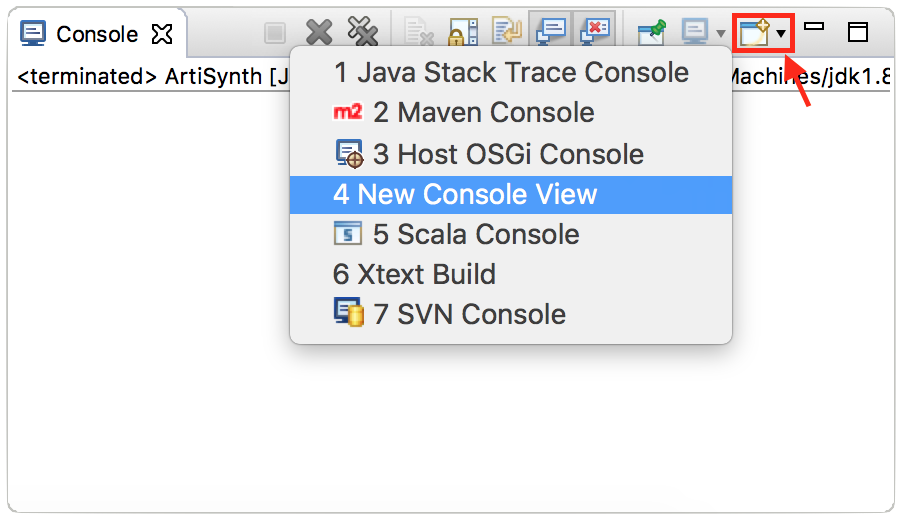
\includegraphics[]{images/batch-worker-launch-1}
\else
 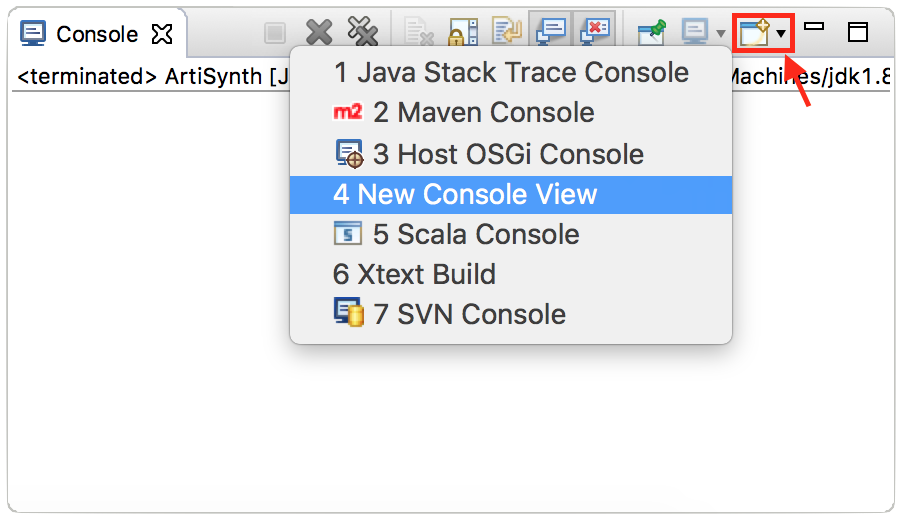
\includegraphics[width=6in]{images/batch-worker-launch-1}
\fi
\end{center}
\caption{Creating a new Console View in Eclipse.}
\label{fig:new-console}
\end{figure}

Next, return to the original console (where the \BM\ is running), and select the {\sf Pin Console} icon (a window with a green pin) in the top-right corner (see Figure \ref{fig:pin-console}). This will pin the \BM\ process to that console. Finally, run the desired \BW\ by running ArtiSynth with the appropriate command line arguments for the \BW\ ({\sf Run As > Run Configurations... > Arguments > Program Arguments > Apply > Run}). Subsequently, the \BW\ can be started like any other Java program in Eclipse. Repeat this step whenever new command line arguments are desired.

\begin{figure}[t]
\begin{center}
\iflatexml
 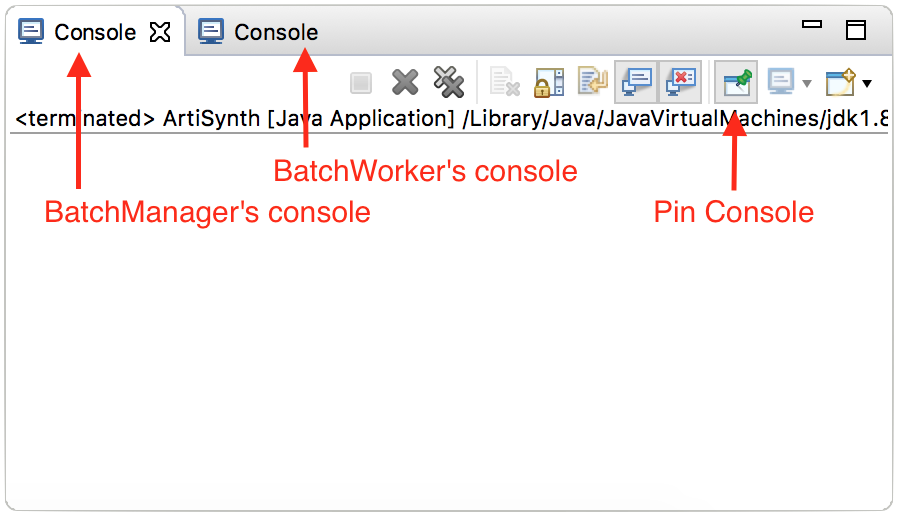
\includegraphics[]{images/batch-worker-launch-2}
\else
 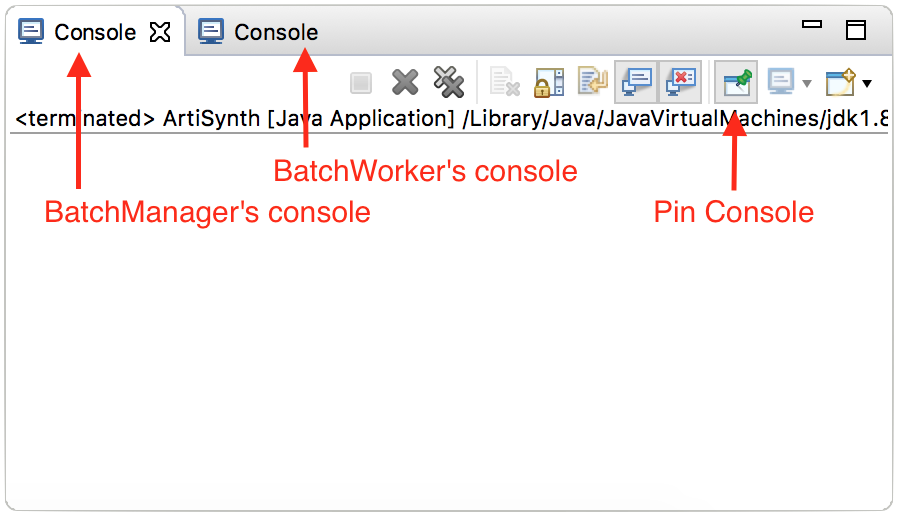
\includegraphics[width=6in]{images/batch-worker-launch-2}
\fi
\end{center}
\caption{Pinning a Console View in Eclipse.}
\label{fig:pin-console}
\end{figure}

\begin{sideblock}
Note: running more than one \BW\ from within Eclipse is not recommended, because Eclipse does not differentiate between instances of the same program when it comes to pinning program outputs in the Console Views. As such, the output from all but one \BW\ will not be visible in the Console Views (the program \textbf{will} run, but not in an accessible fashion). 
\end{sideblock}

\begin{sideblock}
Note: BatchSim can also run using both of Eclipse and the command line. For example, the \BM\ can run in Eclipse, while the $n$ \BWs\ can run from the command line.
\end{sideblock}

\subsection{Advanced BatchSim options}

The preceding examples for running BatchSim (from the command line or from within Eclipse) present only the simplest and most common use case, and allows BatchSim to run in its default mode. Additional modes and behaviours can be specified by appropriate command line arguments.

\subsubsection{Options to the \BM}

At the time of writing, the options for the \BM\ are

\begin{description}

\item[{\tt -h,-help} ] \mbox{}

Prints a help message and exits.

\item[{\tt -f,-file <FILENAME>} ] \mbox{}

Reads the input configurations from file {\tt FILENAME}, which defaults to {\tt props.psl} in the current working directory. If {\tt FILENAME} is {\tt -}, reads from standard input (which forces an interaction level of 0; see {\tt -i} option).

\item[{\tt -m,-monteCarlo <N>} ] \mbox{}

If the input file (see {\tt -f} option) contains \textbf{only} probabilistic specifications, performs {\tt N} \href{https://en.wikipedia.org/wiki/Monte_Carlo_method}{Monte Carlo} (i.e. random/probabilistic) simulations (see Section XXXXXXXXX PSL:prob). Otherwise, this option is ignored. {\tt N} defaults to 1.

\item[{\tt -p,-port <PORT>} ] \mbox{}

Binds the port to which the \BM\ socket is listening for requests from a \BW\ to {\tt PORT}, which defaults to 34365.

\item[{\tt -i,-interactionLevel <LEVEL>} ] \mbox{}

Sets the level of interaction with the user to {\tt LEVEL}, which defaults to 2 (unless {\tt -f -} is given; see {\tt -f} option). A \BM\ can run in ``interactive mode'' by initiating an interactive {\tt ArtisynthJythonConsole} session with the user. There are 3 levels of interaction. Level 0 means the \BM\ outputs nothing except error messages. Level 1 means the \BM\ outputs error and warning messages. Level 2 means fully interactive. In the latter mode, several builtin commands allow the user to interact with the \BM. These are

\begin{lstlisting}[]
  commands() -- output this list of commands
  progress() -- output progress information
  quit()     -- exit with status 0
  quit(st)   -- exit with status `st'
\end{lstlisting}

\item[{\tt -v,-debug} ] \mbox{}

Prints debugging (i.e. verbose) messages. This is independent of the interaction level (see {\tt -i} option).

\item[{\tt -r,-dryRun} ] \mbox{}

Reads the input file (see {\tt -f} option) and exits. This ensures the input file can be parsed without errors.

\item[{\tt -b,-bufferCap <CAP>} ] \mbox{}

Sets the maximum capacity of the buffer used to store created but unsent simulation tasks to {\tt CAP}. This is essentially the maximum size of the \BM's ``bag of tasks.'' {\tt CAP} defaults to $2^{20}$ (just over 1 million), but can be set to a larger value if more than that many simulations tasks will be created and the user is interested in knowing the exact number of simulations to be performed before running them all. On the other hand, it can be set to a smaller value if so many simulation tasks are being created that the JVM runs out of memory and crashes.

\item[{\tt -c,-checkProps} ] \mbox{}

If the \BM\ is running within an instance of ArtiSynth, verifies that the \textbf{currently-loaded} model has all the {\tt Properties} listed in the input file (see {\tt -f} option), and that, for each such {\tt Property}, all the listed values are assignable to that {\tt Property} (see Section \ref{run:bm}).

\item[{\tt -d,-delimiter <CHAR>} ] \mbox{}

Sets the value delimiter character (see Section XXXXXXXXXXXX) of the input file (see {\tt -f} option) to {\tt CHAR}, which defaults to {\tt \%}. Note that some characters are not allowed as the delimiter character. These include any character that already has special syntactic significance, such as {\tt =} or {\tt "} (see {\tt -o} option; see Section XXXXXXXX), as well as digit and whitespace characters.

\item[{\tt -o,-riskyDelimOk} ] \mbox{}

Allows the use of delimiter characters (see {\tt -d} option) that are otherwise too risky to use, because they already have syntactic significance (see Section XXXXXX). Using risky delimiters may require escape characters (see Section XXXXXXX). At the time of writing, the illegal characters are: {\tt \{}, {\tt \}}, {\tt [}, {\tt ]}, {\tt \#}, {\tt (}, {\tt )}, and all digit and whitespace characters. At the time of writing, the risky characters are: {\tt =}, {\tt \textasciitilde}, {\tt "}, {\tt '}, {\tt @}, and {\tt \$}.

\item[{\tt -e,-epsilon <EPS>} ] \mbox{}

Sets the epsilon for comparing two doubles for equality to {\tt EPS}, which defaults to 0.0001.

\item[{\tt -s,-seed <SEED>} ] \mbox{}

Sets the seed for the random number generator to {\tt SEED}, or use no seed at all if {\tt SEED} is -1. {\tt SEED} defaults to -1.

\end{description}

\subsubsection{Options to \BWs}

At the time of writing, the options for each \BW\ are

\begin{description}

\item[{\tt -h,-help} ] \mbox{}

Prints a help message.

\item[{\tt -n,-workerName <NAME>} ] \mbox{}

Sets the \BW's name to {\tt NAME}, which defaults to {\tt worker<PORT>}, where {\tt PORT} is supplied by the {\tt -p} option (or its default runtime value; see {\tt -p} option). Setting a unique name for each \BW\ is important, as it creates a one-to-one correspondence between each \BW\ and its output files, which prevents data corruption and facilitates post-processing (see {\tt -d}, {\tt -l}, and {\tt -f} options; see Section XXXX POSTPROC).

\item[{\tt -d,-outputDirName <DIRNAME>} ] \mbox{}

Sets the \BW's output directory to {\tt DIRNAME}, which defaults to the current working directory. Having unique \BW\ names (see {\tt -n} option) allows each worker to have its own (uniquely named) output file (see {\tt -l} and {\tt -f} options), and yet for all \BWs\ to share a single output directory. Having separate output files is critical to avoid data corruption, and sharing an output directory makes post-processing easier (see Section XXX POST).

\item[{\tt -e,-rerunSims <LIST>} ] \mbox{}

If a simulation fails, reruns that simulation using the time steps listed in {\tt LIST} until success is achieved. {\tt LIST} should be of the form {\tt <double>[[,...],<double>]} (a comma-separated list of doubles given as a single string). {\tt LIST} defaults to the empty list, meaning simulations are not rerun. Certain models, especially those containing finite-element models, are quite unstable and tend to cause simulation crashes. In this case, rerunning the simulation with one-tenth of the original time step can often increase stability enough to resolve the crash. However, running every simulation at that time step is not ideal, since smaller time steps require significantly more computation time. Hence the existence of this option. Since rerunning at one-tenth of the original time step is not always desired, providing a list of arbitrary doubles renders this options far more general.

\item[{\tt -l,-logFileName <FILENAME>} ] \mbox{}

Sets the \BW's log file name to {\tt FILENAME}, which defaults to {\tt <worker\_name>\_log.txt}, where {\tt worker\_name} is supplied by the {\tt -n} option. The log file is intended to store per-simulation logging information. Making use of this file is at the user's discretion (see Section XXXXXXXX).

\item[{\tt -f,-propValFileName <FILENAME>} ] \mbox{}

Sets the \BW's {\tt Property} value file name to {\tt FILENAME}, which defaults to {\tt <worker\_name>\_propVal.txt}, where {\tt worker\_name} is supplied by the {\tt -n} option. The {\tt Property} value file is intended to store the input configuration (i.e. value of each {\tt Property} in the simulation task) used for each simulation run by that \BW. Making use of this file is at the user's discretion (see Section XXXXXXXX).

\item[{\tt -p,workerReplyPort <PORT>} ] \mbox{}

Sets the \BW's \textbf{base} reply port to {\tt PORT}, which defaults to 23159. Note that the actual port used may be different if the port {\tt PORT} is already in use. In this case, the \BW\ will try binding each successive port (incrementing by one) until a port is successfully bound. This incrementing feature is extremely useful in practice, since starting $n$ \BWs\ will automatically cause $n$ successive ports to be bound, without having to explicitly pass a different port number to each \BW. In addition, since \BW\ names and log files (see {\tt -n}, {\tt -l}, and {\tt -f} options) are linked to the port number (by default), this feature ensures unique file names for each \BW\ by default (see {\tt -d} option).

\item[{\tt -m,managerHostName <HOSTNAME>} ] \mbox{}

Informs the \BW\ that the \BM's host machine's name is {\tt HOSTNAME}, which defaults to the \BW's localhost name or loopback address name (by default, BatchSim assumes the network connection is between the \BM\ and the \BWs\ is local).

\item[{\tt -r,managerRequestPort <PORT>} ] \mbox{}

Informs the \BW\ that the \BM\ is listening for requests on port number {\tt PORT}, which defaults to 34365.

\end{description}

\begin{sideblock}
Note: custom \BWs\ can be given additional options (see Section XXXXXXXXXXXXXXX).
\end{sideblock}

\begin{sideblock}
Note: running their respective program with the {\tt -help} option prints a summary of available options for both the \BM\ and \BWs.
\end{sideblock}

\begin{sideblock}
Note: for additional details, consult the Javadocs for \javaclass[artisynth.tools.batchsim]{BatchWorkerBase} and \javaclass[artisynth.tools.batchsim.manager]{BatchManager}.
\end{sideblock}

\section{The Property Specification Language}

Whereas \BWs\ are specifically designed to be customizable, the \BM\ is a complete program that is not intended to be modified. Instead, the \BM's behaviour is modified through the contents of the input file it receives from the user. This file contains the input configuration of every simulation that BatchSim should run. These configurations are provided in a compact form in which the user specifies the values or probability distributions of various {\tt Properties} of a target model, which are known as property specifications. Properties specifications are written in a very simple programming language called the Property Specification Language (PSL).

\subsection{The target model and {\tt Properties}}

BatchSim is model-agnostic in the sense that it can run simulations for any {\tt RootModel} subclass, which BatchSim refers to as the target model. Like much of the ArtiSynth and Maspack codebases, this agnosticism is achieved by accessing model attributes through ArtiSynth's {\tt Property} mechanism, which is very general and widely used. Frequently, the input parameters that are to vary with each simulation are already {\tt Properties}, either of the target model itself, or else of one of its subcomponents (e.g. a finite-element model). Whenever an input parameter is not already a {\tt Property} of some component in the target model's component hierarchy, a {\tt Property} can readily be defined to ``wrap'' said input parameter so as to become a {\tt Property}. Refer to the {\tt Maspack Reference Manual} for details on adding custom {\tt Properties} to any class, including a {\tt RootModel} subclass.

\subsection{Property paths}

Throughout this document, the terms ``property'', ``{\tt Property}'', and property path are used interchangeably and refer to both {\tt Properties} and property paths. A property path is simply a path from the target model to one of its subcomponents, followed by {\tt :}, followed by the name of a {\tt Property} of that component. For {\tt CompositeProperties}, sub-{\tt Properties} can be referenced by separating the name of the {\tt CompositeProperty} and its sub-{\tt Properties} with {\tt .} (a period). Refer to the {\tt Maspack Reference Manual} for details on property paths.

\subsection{Simulation tasks and property-value pairs}

The \BM\ parses the input file and collects all property specifications listed therein. It then processes these property specifications in one of three ways (see Sections XXX, XXX, XXX) to create simulation tasks. Each simulation task contains a list of {\tt Properties} and, for each, a particular value to which it should be set for that particular simulation. These are known as property-value pairs. Each value is a textual (i.e. string) representation of a value that can be assigned to the associated {\tt Property}. The format of this string must be such that the {\tt PropertyInfo.scanValue(ReaderTokenizer)} method can scan it.

There are two kinds of property specifications: combinatorial and probabilistic. As part of the property specification, the user either hardcodes the {\tt Property} values directly to create a combinatorial specification (see Section XXXXXX), or else indicates the probability distribution from which to draw the values to create a probabilistic specification (see Section XXXXX).

\subsection{Combinatorial property specifications}

Here, a particular {\tt Property} is associated with a \textit{set} of values, and each value is assigned to the {\tt Property} in turn during successive simulations. Other {\tt Properties} are associated with different value sets in their own combinatorial specification. The \BM\ iterates through the values in all combinatorial specifications so as to perform an exhaustive search of the input space: each possible combination of property-value pairs for all combinatorial specifications is examined. Each simulation task consists of exactly one such combination. More formally, say there are $N$ such combinatorial specifications. Then, the general exhaustive-search/combinatorial algorithm is

\begin{lstlisting}[]
  for value1 in specification1.valueSet()
     for value2 in specification2.valueSet()
        // ...
           for valueN in specificationN.valueSet()
              createSimulationTask(value1, value2, ..., valueN)
           endFor
        // ...
     endFor
  endFor
\end{lstlisting}

\begin{sideblock}
Note: the actual algorithm is recursive (where {\tt // ...} represents the recursion), but it is easier to understand this ``unfolded'' version.
\end{sideblock}

\begin{sideblock}
Note: mathematically speaking, one simulation task is performed for each element in the $N$-ary \href{https://en.wikipedia.org/wiki/Cartesian_product}{Cartesian product} of all the value sets.
\end{sideblock}

\subsection{Probabilistic property specifications}

Here, a particular \textbf{numeric} {\tt Property} is associated with a \textit{vector} of parametric probability distributions, with the size of the probability distribution vector equal to the size of the {\tt Property} vector. For a scalar numeric {\tt Property}, the probability distribution vector should contain a single entry. Other {\tt Properties} are associated with different probabilistic distribution vectors in their own probabilistic specification. If \textbf{only} probabilistic specifications are given, the manager creates simulation tasks by applying the Monte Carlo method. That is, for each probabilistic specification, all the distributions listed in its associated probability distribution vector are sampled, and a random-value vector is formed from the sampled values. These sampled vectors are then assembled into one simulation task (thus forming one Monte Carlo simulation task), and the process is repeated $M$ times, where $M$ is specified by the user (see the {\tt -m} option of the \BM\ in Section XXXXXXXXXX). Formally, the algorithm is

\begin{lstlisting}[]
  for i in 1 to M
     vectors = new List()
     for specification in specificationsList
        sampledVector = new Vector()
        for distribution in specification.distributionVector()
           sampledVector.add(distribution.sample())
        endFor
        vectors.add(sampledVector)
     endFor
     createSimulationTask(vectors)
  endFor
\end{lstlisting}

\subsection{Running hybrid combinatorial/probabilistic simulations}

If at least one probabilistic specification and at least one combinatorial specification are given, the combinatorial algorithm described above is used, but augmented with a check for the specification's type. If the specification is probabilistic, it is treated as if its distribution vector was a single combinatorial value (whose value just happens to be different with each combination). The end result is a hybrid algorithm between exhaustive-search/combinatorial and Monte Carlo, which is described by the following algorithm

\begin{lstlisting}[]
  iterator = specificationsList.iterator()
  while iterator.hasNext()
     specification1 = iter.next()
     if specification1.type() is COMBINATORIAL
        for value in specification1.valueSet()
           specification2 = iterator.next()
           // ...
              createSimulationTask(value, ...)
           // ...
        endFor
     else // specification1.type() == PROBABILISTIC
        sampledVector = new Vector()
        for distribution in specification1.distributionVector()
           sampledVector.add(distribution.sample())
        endFor
        specification2 = iterator.next()
        // ...
           createSimulationTask(sampledVector, ...)
        // ...
     endIf 
  endWhile
\end{lstlisting}

\begin{sideblock}
Note: again, the actual algorithm is recursive (where {\tt // ...} represents the recursion), but it is \textit{much} easier to understand this ``unfolded'' version.
\end{sideblock}

\subsection{Property specifications}

\subsubsection{Property path syntax}

Whether combinatorial or probabilistic, each property specification begins with a double-quoted property path

\begin{lstlisting}[]
  "<property_path>"
\end{lstlisting}

where {\tt <property\_path>} must be a valid ArtiSynth property path, except for an optional component identifier set extension provided by BatchSim that allows multiple components to be grouped into a single specification (see Section XXXXXXXXXX).

\subsubsection{Combinatorial specification syntax}

Each combinatorial specification must adhere to the following general format

\begin{lstlisting}[]
  "<property_path>" = <value_set>
\end{lstlisting}

where {\tt <value\_set>} must be of the form

\begin{lstlisting}[]
   { <delim><val1><delim> <delim><val2><delim> ... <delim><valN><delim> }
\end{lstlisting}

where {\tt <delim>} is a chosen value delimiter character ({\tt \%} by default; see the {\tt -d} option of the \BM\ in Section XXXXXXXXXX). Each {\tt <valX>} consists of the entire string between two consecutive occurrences of {\tt <delim>} (including all whitespace except the end-of-line character; see Section XXXXXXXX), and is taken to represent a single (presumably valid) value for the associated {\tt Property}.

Some examples of valid combinatorial property specifications (when the delimiter character is the default {\tt \%}) are

\begin{lstlisting}[]
  "models/0/component/1:someProp.someSubProp" = {%1% %2% %3%}
  "color" = {%"red"% %"green"%}
  "someVectorProp" = {%[1 2 3]% %[4 5 6]%}
\end{lstlisting}

\begin{sideblock}
Note: the preceding example involving the {\tt "color"} property path illustrates why the default delimiter character is {\tt \%} instead of {\tt "} (double quote): if a {\tt Property}'s type is {\tt String}, the {\tt ReaderTokenizer} input to the {\tt PropertyInfo.scanValue(ReaderTokenizer)} method must be fed a double-quoted string, which means the values of this property specification would have had to be coded as {\tt ""red""} and {\tt ""green""} if {\tt "} was the delimiter character. Clearly, this will not be parsed correctly. Similar arguments apply to using {\tt '} or {\tt ,} as the default delimiter character.
\end{sideblock}

\begin{sideblock}
It \textbf{\textit{is}} possible to set the delimiter character to {\tt "}, but in this case the quotes belonging in the value need to be escaped: {\tt "\textbackslash"red\textbackslash""} and {\tt "\textbackslash"green\textbackslash""}. This also requires passing the {\tt -o} option to the \BM\ (see Section XXXXXXXX).
\end{sideblock}

\subsubsection{Probabilistic specification syntax}

Each probabilistic specification must adhere to the following general format

\begin{lstlisting}[]
   "<property_path>" ~ <distribution_vector>
\end{lstlisting}

where {\tt <distribution\_vector>} must be of the form

\begin{lstlisting}[]
   [ <distribution1> <distribution2> ... <distributionN> ]
\end{lstlisting}

where the number of distributions listed between the pair of square brackets must match the size of the associated {\tt Property}'s data type. For scalar-valued {\tt Properties}, a single distribution should be listed. For vector-valued {\tt Properties}, the number of distributions listed should match the vector's size. Each {\tt <distributionX>} must be of the form

\begin{lstlisting}[]
  <Name_of_distribution>(<parameter1_value>, ..., <parameterN_value>)
\end{lstlisting}

where {\tt <Name\_of\_distribution>} is the non-quoted string name of a probability distribution. To be valid, this name must match {\tt Distribution.toString()} for some \javaclass[artisynth.tools.batchsim.manager.DistributionSampler]{Distribution} value. Following the distribution name, a \textit{comma-separated} list of parameter values (integers or doubles, depending on the distribution) enclosed in one pair of parentheses should appear. The values must appear in the same order and be in the same quantity as specified by the corresponding \javaclass[artisynth.tools.batchsim.manager.DistributionSampler]{Distribution}, and each value must be a valid number for that particular parameter of that particular \javaclass[artisynth.tools.batchsim.manager.DistributionSampler]{Distribution}. 

Some examples of valid probabilistic property specifications are

\begin{lstlisting}[]
  "models/0/component/1:someScalarProp" ~ [ Normal(20.0, 1.5) ]
  "colorRGB" ~ [ Uniform(0, 1) Uniform(0, 1) Uniform(0, 1) ]
  "someVectorPropWithConstant2ndEntry" ~ [
     T(2)
     Uniform(1, 1)
     Normal(0, 1)
  ]
\end{lstlisting}

\begin{sideblock}
Aside: in probabilistic specifications, {\tt \textasciitilde} is borrowed from probability theory notation: if a random variable $X$ is distributed according to a probability distribution $D$, then we write $X$ \textasciitilde\ $D$. Here, we augment this notation by using $\textbf{X}$ (the {\tt Property}) to represent a vector of random variables, and we specify one probability distribution, $D_i$, for each entry $i$ of $\textbf{X}$, notated as $\textbf{X}$ \textasciitilde\ [$D_1$ $D_2$ ... $D_n$].
\end{sideblock}

\subsubsection{General syntax}

Some notes on the input file syntax (in terms of tokens) of property specifications follow. Unless otherwise indicated, syntax rules apply to both types of property specifications.

\begin{enumerate}

\item The {\tt \#} token begins a comment. All characters between it and the next end-of-line character are ignored.

\item The {\tt <property\_path>} token must be double-quoted.

\item All tokens in any specification can be separated by an arbitrary number of whitespace characters. Thus, the following examples are all syntactically valid and semantically equivalent combinatorial property specifications

\begin{lstlisting}[]
  "models:prop" = { %val1% %val2% }
  "models:prop" = {%val1% %val2%}
  "models:prop"={%val1%%val2%}
  "models:prop" = {
     %val1%
     %val2%
  }
\end{lstlisting}

\item The value set of a combinatorial specification \textit{can} be empty: {\tt \{\}}. In this case, but only in this case, the associated {\tt Property} will be assigned the value {\tt null} in all simulation tasks.

\item Whitespace appearing in any double-quoted string will be considered part of the string token, \textbf{unless} it is an end-of-line character, which will cause the string to be split into multiple word tokens. This applies to value strings delimited by the delimiter character as well ({\tt \%} by default), and is caused by the \javaclass[maspack.util]{ReaderTokenizer} used to parse the input file. One exception to this rule is that non-end-of-line whitespace appearing \textit{within a component identifier set} of a {\tt <property\_path>} token is ignored (see Section XXXXXXXXXXX).

\end{enumerate}

\subsubsection{Component identifier sets}

Within the {\tt <property\_path>}, a special set notation can be used as a shorthand to group multiple subcomponents of a particular component into a single specification. This is useful if some or all subcomponents would otherwise be specified as having the same value set (for combinatorial specifications) or the same distribution vector (for probabilistic specifications).

Within the {\tt <property\_path>}, instead of a single component name or number (collectively called a component identifier), a \textit{set} of identifiers can be specified (within a pair of curly braces). This set will be ``expanded'' in place by creating one (implicit) specification for each component identifier in the set. For example, the {\tt <property\_path>}

\begin{lstlisting}[]
  "models/{mySubComponent1 mySubComponent2}:prop"
\end{lstlisting}

will be expanded into

\begin{lstlisting}[]
  "models/mySubComponent1:prop"
  "models/mySubComponent2:prop"
\end{lstlisting}

This expansion works regardless of the property specification type: the value set (for combinatorial specifications) or distribution vector (for probabilistic specifications) is copied (re-instantiated) for each expanded {\tt <property\_path>}.

\begin{sideblock}
Note: the individual identifiers in a component identifier set must be separated by an arbitrary number of non-end-of-line whitespace characters.
\end{sideblock}

\begin{sideblock}
Note: since a component identifier set appears within a {\tt <property\_path>}, which is itself quoted by {\tt "}, it cannot contain {\tt "} characters anywhere.
\end{sideblock}

\begin{sideblock}
Note: since components cannot be identified without an identifier, a component identifier set cannot be empty.
\end{sideblock}

Since the unique number of any ArtiSynth subcomponent is an integer, an \textit{inclusive} \textbf{range} of such integers can be provided as yet an another shorthand. For example, the {\tt <property\_path>}

\begin{lstlisting}[]
  "models/{[0-2] [24-25]}:prop"
\end{lstlisting}

will be expanded into

\begin{lstlisting}[]
  "models/0:prop"
  "models/1:prop"
  "models/2:prop"
  "models/24:prop"
  "models/25:prop"
\end{lstlisting}

\begin{sideblock}
Note: an arbitrary number of whitespace characters can separate the individual characters within the range.
\end{sideblock}

\begin{sideblock}
Note: the first integer specified in a range must be less than or equal to the second integer in the range, but separate ranges need not be listed in increasing order.
\end{sideblock}

The expansion of a component identifier is done in place, i.e. the substring delimited by the curly braces will be exactly replaced by each identifier listed in the set. For example, the {\tt <property\_path>}

\begin{lstlisting}[]
  "models/comp{   [0-2] [24-25] }onent:prop"
\end{lstlisting}

will be expanded into

\begin{lstlisting}[]
  "models/comp0onent:prop"
  "models/comp1onent:prop"
  "models/comp2onent:prop"
  "models/comp24onent:prop"
  "models/comp25onent:prop"
\end{lstlisting}

and the {\tt <property\_path>}

\begin{lstlisting}[]
  "models/{ left right top }_comp:prop"
\end{lstlisting}

will be expanded into

\begin{lstlisting}[]
  "models/left_comp:prop"
  "models/right_comp:prop"
  "models/top_comp:prop"
\end{lstlisting}

The identifiers in a component identifier set can in fact be component paths or path fragments as well. For example, the {\tt <property\_path>}

\begin{lstlisting}[]
  "models/{comp0/1 comp2/3}:prop"
\end{lstlisting}

will be expanded into

\begin{lstlisting}[]
  "models/comp0/1:prop"
  "models/comp2/3:prop"
\end{lstlisting}

Finally, multiple \textit{sequential} component identifier sets can be specified within a single {\tt <property\_path>}, and these will be expanded in a combinatorial fashion. For example, the {\tt <property\_path>}

\begin{lstlisting}[]
  "models/comp{0 1}/{2 3}:prop"
\end{lstlisting}

will be expanded into

\begin{lstlisting}[]
  "models/comp0/2:prop"
  "models/comp0/3:prop"
  "models/comp1/2:prop"
  "models/comp1/3:prop"
\end{lstlisting}

However, at the time of writing, BatchSim does \textbf{not} support nested component identifier sets. For example, the {\tt <property\_path>}

\begin{lstlisting}[]
  "models/comp{[0-1] {2 3}}:prop"
\end{lstlisting}

is \textbf{\textit{not}} valid and will not be expanded.

\subsubsection{Decorators}

Sometimes, it may be useful to specify a property specification as probabilistic, but then pre-sample from its distribution vector a certain number of times, say $k$, and treat these $k$ values as though they were values in a combinatorial value set. In other words, the property specification is specified as probabilistic, but we sample from it $k$ times, and then treat the resulting values as the $k$ values of the value set of a combinatorial property specification.

Similarly, we may want to specify as property specification as combinatorial, but instead of iterating deterministically through its value set to created simulation tasks, we may want to randomly sample from this set. Furthermore, we may want each value to have a different probability of being sampled. In other words, the property specification is specified as combinatorial, but we treat its value set as the support of a discrete probability distribution, and then sample from this distribution as if the property specification was probabilistic.

BatchSim supports both of these features through ``decorators.'' As the name implies, these objects decorate a property specification to modify its interpretation. The syntax is as follows. For combinatorially-decorated probabilistic specifications

\begin{lstlisting}[]
  @COMB(k) <probabilistic_property_specification>
\end{lstlisting}

leads to sampling the distribution vector of the property specification $k$ times.

\begin{sideblock}
Note: to have repeatable results, consider fixing the seed of the \BM's random number generator (see {\tt -s} option to the \BM\ in Section XXXXXXXXXX).
\end{sideblock}

For probabilistically-decorated combinatorial specifications

\begin{lstlisting}[]
  @PROB <combinatorial_property_specification>
\end{lstlisting}

leads to uniform sampling of the value set, while

\begin{lstlisting}[]
  @PROB(p1, p2, ..., pN) <combinatorial_property_specification>
\end{lstlisting}

leads to sampling with value-specific probabilities. Here, the usual constraints on discrete probability distributions, namely $\Sigma{p_i} = 1$ and $p_i \geq 0$, $i = 1,2,\dots,N$, must hold.

\begin{sideblock}
Note: the first form is just a shorthand for the second form, with $p_i = \frac{1}{N}$, $i = 1,2,\dots,N$.
\end{sideblock}

\begin{sideblock}
Note: the number of values in the value set must match the number of arguments to the {\tt @PROB} decorator.
\end{sideblock}

Sometimes it may be useful to have a property specification that exists solely for triggering control structures (see Section XXXXXXXX), rather than as a simulation input. But property specifications that don't correspond to a real {\tt Property} in the target model result in the \BWs\ throwing a runtime error. The only way around this would be to add a new ``phony'' {\tt Property} to the target model. This is obviously not very elegant and needlessly clutters the target model's code. Instead, a third kind of decorator exists, the {\tt @PHONY} decorator, which simply flags the property specification as phony. The \BM\ never passes any phony {\tt Properties} to the \BWs, which resolves the runtime error problem, but the property specification can still be used in the input file to trigger control structures.

\begin{sideblock}
Note: any property specification (whether otherwise decorated or not) can be \textbf{prepended} by at most one {\tt @PHONY} decorator.
\end{sideblock}

\begin{sideblock}
Note: at the time of writing, BatchSim does not support the addition of multiple {\tt @PROB} or {\tt @COMB} decorators to a single property specification.
\end{sideblock}

\subsection{Control structures}

At the time of writing, property specifications can be affected by three control structures: {\tt skip} statements, {\tt redef} (i.e. redefinition) statements, and Jython code blocks. These structures are useful for removing certain combinations of input values that would otherwise be discarded as invalid simulations in post-processing. The power of using these structures comes from the fact that they save valuable computation time by not running simulations that will end up being discarded anyways. In addition, they simply post-processing, because discarding specific pieces of data later on may be non-trivial, and may require manual intervention (although this depends on how the output data is recorded).

\begin{sideblock}
Note: because they can interact in complex and very subtle ways, very little checking is done to ensure valid use of these control structures prior to running simulations. For example, multiple {\tt redef} statements can ``cascade,'' where one is triggered, which redefines some other {\tt Property}, which later triggers yet another. Although this is valid, and even encouraged in many cases, no checks are made to ensure nothing is done incorrectly. Instead, task creation proceeds assuming everything will work out, and only if an error is detected during task creation will a meaningful error message be given.
\end{sideblock}

\subsubsection{{\tt skip} statements}

A {\tt skip} statement is a list of \textit{combinatorial} property specifications, each of which has to have a property path that has already been defined at some earlier point in the input file (possibly with a different value set; the ``identity'' of property specifications is tied to the property path). A {\tt skip} statement causes simulations to be skipped. Specifically, it skips all simulations where each of the {\tt Properties} listed in the {\tt skip} statement has a current value equal to any one of the values listed in its value set. That is, multiple property specifications listed together in the same {\tt skip} statement are logically ANDed, and, within each property specification, the values in its value set are logically ORed. This is called a {\tt skip} match. The syntax of a {\tt skip} statement is the keyword {\tt skip} followed by a list of \textbf{undecorated, combinatorial} property specifications (called the {\tt skip} block), followed by the keyword {\tt end}. For example

\begin{lstlisting}[]
  "prop1" = {%0% %1% %2%}
  "prop2" = {%3% %4% %5%}
  skip
     "prop1" = {%1% %2%}
     "prop2" = {%3% %4%}
  end
\end{lstlisting}

will skip all simulations where ({\tt "prop1"} = {\tt 1} OR {\tt "prop1"} = {\tt 2}) AND ({\tt "prop2"} = {\tt 3} OR {\tt "prop2"} = {\tt 4}), but allow all others (i.e. the pairs ({\tt 0}, {\tt 3}), ({\tt 0}, {\tt 4}), ({\tt 0}, {\tt 5}), ({\tt 1}, {\tt 5}), and ({\tt 2}, {\tt 5}) are all allowed).

\subsubsection{{\tt redef} statements}

{\tt redef} statements are composed of two blocks. The syntax is the keyword {\tt redef} followed by a list of property specifications, which may be combinatorial or probabilistic, and decorated or not (called the {\tt redef} block), followed by the keyword {\tt when}, followed by a list of \textbf{undecorated, combinatorial} property specifications (called the {\tt when} block), followed by the keyword {\tt end}.

The {\tt when} block is similar to the {\tt skip} block of the {\tt skip} statement, except that instead of skipping simulation tasks that match the block, it triggers the redefinition of the property specification(s) in the {\tt redef} block. ``Redefinition'' means that the property path stays the same, and so refers to the same {\tt Property} of the target model, but some other part of the property specification changes. The change can be anything: adding a decorator, changing the values in the value set, changing the probability distributions in a distribution vector, changing the size of the value set or distribution vector, changing the property specification from combinatorial to probabilistic, or anything else.

A list of these redefinable property specifications should appear in the {\tt redef} block. This list is just a shorthand: implicitly, there is one separate and completely independent redefinition for each property specification listed in the {\tt redef} block. As such, it would be equivalent to having one redefinition with the same {\tt when} block for each property specification listed in the {\tt redef} block. One catch: \textbf{every} property specification listed in the {\tt redef} block must be initially defined (in the input file) \textbf{after} every specification listed in the {\tt when} block.

\begin{sideblock}
Aside: we can think of the contents of the input file as a directed graph where each property specification is a node, and where there is a directed edge from one property specification to another if the former appears immediately before the latter in this file. Then, a topological sort of the resulting directed acyclic graph (DAG) would place the property specifications in the same order as they appear in the input file. With this in mind, we can think of a {\tt redef} statement as introducing several more directed edges to the DAG. Each such edge starts at a property specification in the {\tt when} block and ends at a property specification in the preceding {\tt redef} block. The {\tt redef} statement, then, is valid if and only if the graph that results from the introduction of these new edges is still a DAG (i.e. has no cycles). This is done to prevent cyclical redefinitions, which are usually hard to get right, and often cause infinite loops unless extreme care is taken to avoid them.
\end{sideblock}

{\tt redef} statements become extremely useful when combined with {\tt @PHONY} property specifications that act as flags. For example, in

\begin{lstlisting}[]
  @PHONY "prop1" = {%LOW% %HIGH%}
  "prop2" = {} # I.e. prop2 is set to null.
  "prop3" = {%value_for_low% %value_for_high%} # Or could be set to null.
  redef
     "prop2" = {%1% %2%}
     "prop3" = 
  when
     "prop1" = 
  end
  redef
     "prop2" = {%9% %10%}
     "prop3" = 
  when
     "prop1" = 
  end
\end{lstlisting}

{\tt "prop1"} acts as a flag which makes some other properties, namely {\tt "prop2"} and {\tt "prop3"}, have values that are either low or high in tandem. This effectively skips simulations where one has a low value while the other has a high value, which (in this example) we would want to discard as invalid.

\begin{sideblock}
Note: since the effect of {\tt skip} and {\tt redef} statements is the same (discarding unwanted simulations), these two structures are effectively equivalent. Indeed, they simply represent different ways of expressing the same discard behaviour/logic, and one can always be defined in terms of the other. However, since the logic may be much more complicated to express with one compared to the other, both are made available for convenience.
\end{sideblock}

\subsubsection{Jython code blocks}

Jython code blocks are different from {\tt skip} and {\tt redef} statements in that they are not standalone statements. Instead, they must occur within a {\tt skip} or {\tt when} block. They act as an additional way in which {\tt skip} or {\tt when} matches can be detected. This can be useful, for example, to match conditional on the value of a probabilistic property specification, which are not allowed in {\tt skip} and {\tt when} blocks. In fact, Jython code blocks can entirely replace the combinatorial matching described above. The advantage of the combinatorial matching, however, is in terms of (1) a convenient syntax, and (2) \textbf{noticeably faster computation time} on the part of the \BM\ (the \BWs\ are unaffected).

\begin{sideblock}
Note: the computational slowdown comes from the fact that, rather than executing everything in Java, the \BM\ has to load the Jython code into a Jython interpreter and then relinquish control to the interpreter, which runs the Jython code before eventually returning control to the \BM.

\textbf{Although the computational slowdown is noticeable, it is \textit{rarely} significant enough to cause problems.} This is because the \BM\ creates simulation tasks (to fill its bag of tasks) in a separate thread than the one listening for task requests from the \BWs. A slowdown will therefore only affect the overall speed of BatchSim if simulation runtimes are faster than task creation times. This is very unlikely, unless the target model is extremely simple and there are a lot of Jython code blocks in the input file.
\end{sideblock}

The syntax of a Jython code block is the keyword {\tt jython} followed by a list of arbitrary lines of Jython code, each of which must be prepended by a {\tt \$}, followed by the keyword {\tt end}. Within the Jython code, two special functions are exposed.

\begin{description}

\item[{\tt get()} ] \mbox{}

Takes a string representing a property path, and returns the current value of the property specification with that property path (as a string), or {\tt None} if the value is not set.

\item[{\tt return\_value()} ] \mbox{}

Takes a boolean and returns nothing. {\tt return\_value(True)} is a callback that passes the given value back to the \BM. If the Jython code block should trigger a match (either in a {\tt skip} or {\tt when} block), then {\tt return\_value(True)} should be called. Otherwise, {\tt return\_value(False)} should be called.

\begin{sideblock}
Note: calling {\tt return\_value()} multiple times within a single Jython code block is not permitted.
\end{sideblock}

\begin{sideblock}
Note: if a {\tt skip} or {\tt when} block contains both Jython code blocks and combinatorial property specifications, then all of them must match for an overall block-level match to be established.
\end{sideblock}

\end{description}

As an example of using Jython code blocks, consider

\begin{lstlisting}[]
  "prop1" = {%0% %1% %2%}
  "prop2" = {%3% %4% %5%}
  skip
     jython
        $prop1_val = get("prop1")
        $return_value(prop1_val in ["1", "2"])
     end
     "prop2" = {%3% %4%}
  end
\end{lstlisting}

This is identical to the example {\tt skip} statement shown in Section XXXXXXXXXX, \textbf{except that it will be computationally slower}.

\begin{sideblock}
Note: Although it may not be apparent in this simple example, the (often slight) computation slowdown of the Jython code blocks may well be worth it, since, in more complicated use cases, using only {\tt skip} or {\tt redef} statements may be extremely cumbersome/bug-prone. In general, {\tt skip} and {\tt redef} statements should be considered ``accelerated'' special cases provided by BatchSim.
\end{sideblock}

In addition to the above Jython code block syntax, Jython one-liners can be specified by appending an additional {\tt \$} to the end of the one line of Jython code (the {\tt end} keyword must still be present). For example, the following is identical to the previous example

\begin{lstlisting}[]
  "prop1" = {%0% %1% %2%}
  "prop2" = {%3% %4% %5%}
  skip
     jython $return_value(get("prop1") in ["1", "2"])$ end
     "prop2" = {%3% %4%}
  end
\end{lstlisting}

\section{Customizing BatchSim}
\label{custom}

Whereas the \BM's behaviour is modified using the input file, the \BWs\ are designed to be customized by sublcassing \javaclass[artisynth.tools.batchsim]{BatchWorkerBase}, which is an abstract class.

1. How BWB works and what sort of customization is possible.

2. Not needed if STBW is enough.

3. BW (\& Jython script)

\section{Post-processing}

1. Need RM. Need {\tt Properties} that match {\tt props.psl}.

2. Need BW.  Alternatively, a "default" \BW\ subclass can be used: {\tt SimpleTimedBatchWorker}, which has a single time stop condition (stopping the simulation after a certain amount of time has elapsed), records the end-state of the model in binary waypoint files, and does some simple logging.

2.1 If using STBW, can use the default jython script: the {\tt batchDriver.py} script can be used to drive the {\tt SimpleTimedBatchWorker}.

3. Props file needs a special default name. Else, additional CLI option needed.

4. Low interactivity of \BM\ is usually coupled to ``no GUI mode.''

5. For repeatable results, set SEED of \BM\ and disable hybrid solves of \BWs.

\begin{lstlisting}[]


   Can also put the return value if it's in Java!!!!!!!!!!!!!!!!!!!!!
   
   
   
   

   iprobeToMatlab (probeName, matlabName)
   iprobeFromMatlab (probeName, matlabName)
   iprobeToMatlab (probeName)
   iprobeFromMatlab (probeName)

   oprobeToMatlab (probeName, matlabName)
   oprobeFromMatlab (probeName, matlabName)
   oprobeToMatlab (probeName)
   oprobeFromMatlab (probeName)
\end{lstlisting}

\end{document}
